% !TEX TS-program = XeLaTeX
% use the following command:
% all document files must be coded in UTF-8
\documentclass[english]{textolivre}
% build HTML with: make4ht -e build.lua -c textolivre.cfg -x -u article "fn-in,svg,pic-align"

\journalname{Texto Livre}
\thevolume{17}
%\thenumber{1} % old template
\theyear{2024}
\receiveddate{\DTMdisplaydate{2022}{12}{19}{-1}} % YYYY MM DD
\accepteddate{\DTMdisplaydate{2023}{10}{31}{-1}}
\publisheddate{\DTMdisplaydate{2023}{11}{27}{-1}}
\corrauthor{Amin Amirdabbaghian}
\articledoi{10.1590/1983-3652.2024.42167}
%\articleid{NNNN} % if the article ID is not the last 5 numbers of its DOI, provide it using \articleid{} commmand 
% list of available sesscions in the journal: articles, dossier, reports, essays, reviews, interviews, editorial
\articlesessionname{articles}
\runningauthor{Kuek et al.} 
%\editorname{Leonardo Araújo} % old template
\sectioneditorname{Daniervelin Pereira}
\layouteditorname{Leonado Araújo}

\title{Users’ quality expectations and their correspondence with the realistic features of translation applications}
\othertitle{Expectativas de qualidade dos usuários e sua correspondência com os recursos realistas dos aplicativos de tradução}
% if there is a third language title, add here:
%\othertitle{Artikelvorlage zur Einreichung beim Texto Livre Journal}

\author[1]{Jing Rou Kuek~\orcid{0009-0008-6441-1550}\thanks{Email: \href{mailto:hazelkuek@ucsiuniversity.edu.my}{hazelkuek@ucsiuniversity.edu.my}}}
\author[2]{Mansour Amini~\orcid{0000-0003-2149-4604}\thanks{Email: \href{mailto:mansour@usm.my}{mansour@usm.my}}}
\author[3]{Ching Sin Siau~\orcid{0000-0001-7612-6839}\thanks{Email: \href{chingsin.siau@ukm.edu.my}{chingsin.siau@ukm.edu.my}}}
\author[4]{Amin Amirdabbaghian~\orcid{0000-0001-6503-8446}\thanks{Email: \href{amirdabbaghian@um.edu.my}{amirdabbaghian@um.edu.my}}}
\affil[1]{UCSI University, Faculty of Social Sciences and Liberal Arts, English Language and Communication Department, Kuala Lumpur, Malaysia.}
\affil[2]{Universiti Sains Malaysia, School of Languages, Literacies, and Translation, Penang, Malaysia.}
\affil[3]{Universiti Kebangsaan Malaysia, Faculty of Health Sciences, Kuala Lumpur, Malaysia.}
\affil[4]{Universiti Malaya, Faculty of Languages and Linguistics, Department of English Language, Malaysia.}

\addbibresource{article.bib}
% use biber instead of bibtex
% $ biber article

% used to create dummy text for the template file
\definecolor{dark-gray}{gray}{0.35} % color used to display dummy texts
\usepackage{lipsum}
\SetLipsumParListSurrounders{\colorlet{oldcolor}{.}\color{dark-gray}}{\color{oldcolor}}

% used here only to provide the XeLaTeX and BibTeX logos
\usepackage{hologo}

% if you use multirows in a table, include the multirow package
\usepackage{multirow}

% provides sidewaysfigure environment
\usepackage{rotating}

% CUSTOM EPIGRAPH - BEGIN 
%%% https://tex.stackexchange.com/questions/193178/specific-epigraph-style
\usepackage{epigraph}
\renewcommand\textflush{flushright}
\makeatletter
\newlength\epitextskip
\pretocmd{\@epitext}{\em}{}{}
\apptocmd{\@epitext}{\em}{}{}
\patchcmd{\epigraph}{\@epitext{#1}\\}{\@epitext{#1}\\[\epitextskip]}{}{}
\makeatother
\setlength\epigraphrule{0pt}
\setlength\epitextskip{0.5ex}
\setlength\epigraphwidth{.7\textwidth}
% CUSTOM EPIGRAPH - END

% LANGUAGE - BEGIN
% ARABIC
% for languages that use special fonts, you must provide the typeface that will be used
% \setotherlanguage{arabic}
% \newfontfamily\arabicfont[Script=Arabic]{Amiri}
% \newfontfamily\arabicfontsf[Script=Arabic]{Amiri}
% \newfontfamily\arabicfonttt[Script=Arabic]{Amiri}
%
% in the article, to add arabic text use: \textlang{arabic}{ ... }
%
% RUSSIAN
% for russian text we also need to define fonts with support for Cyrillic script
% \usepackage{fontspec}
% \setotherlanguage{russian}
% \newfontfamily\cyrillicfont{Times New Roman}
% \newfontfamily\cyrillicfontsf{Times New Roman}[Script=Cyrillic]
% \newfontfamily\cyrillicfonttt{Times New Roman}[Script=Cyrillic]
%
% in the text use \begin{russian} ... \end{russian}
% LANGUAGE - END

% EMOJIS - BEGIN
% to use emoticons in your manuscript
% https://stackoverflow.com/questions/190145/how-to-insert-emoticons-in-latex/57076064
% using font Symbola, which has full support
% the font may be downloaded at:
% https://dn-works.com/ufas/
% add to preamble:
% \newfontfamily\Symbola{Symbola}
% in the text use:
% {\Symbola }
% EMOJIS - END

% LABEL REFERENCE TO DESCRIPTIVE LIST - BEGIN
% reference itens in a descriptive list using their labels instead of numbers
% insert the code below in the preambule:
%\makeatletter
%\let\orgdescriptionlabel\descriptionlabel
%\renewcommand*{\descriptionlabel}[1]{%
%  \let\orglabel\label
%  \let\label\@gobble
%  \phantomsection
%  \edef\@currentlabel{#1\unskip}%
%  \let\label\orglabel
%  \orgdescriptionlabel{#1}%
%}
%\makeatother
%
% in your document, use as illustraded here:
%\begin{description}
%  \item[first\label{itm1}] this is only an example;
%  % ...  add more items
%\end{description}
% LABEL REFERENCE TO DESCRIPTIVE LIST - END


% add line numbers for submission
%\usepackage{lineno}
%\linenumbers

\usepackage{pifont}% http://ctan.org/pkg/pifont
\newcommand{\cmark}{\ding{51}}%
\newcommand{\xmark}{\ding{55}}%

\begin{document}
\maketitle

\begin{polyabstract}
\begin{abstract}
With the accelerating pace of technological developments, translation applications have emerged as the latest trend of machine translation to serve users’ needs for various purposes such as study, work, travel, and entertainment. While the goal of every service, including translation, is to attain user satisfaction, a greater understanding of users’ expectations is essential to improve translation applications and enhance the user experience. This study aims at exploring the users’ quality expectations of translation applications and the realistic features of the applications. A qualitative research design was used to analyze 240 user expectations selected purposefully from 12 popular translation applications. The descriptions given by the developers of the 12 applications were evaluated using \posscite{ryan_machine_1993} model to explore the correspondence between users’ expectations and realistic features of translation applications. The findings revealed a detailed list of quality service criteria and translation quality criteria as well as suggestions to improve both types of criteria. The study may have empirical and theoretical implications for translation researchers and translation application developers in the attempt to compile a comprehensive and realistic profile of translation application features and quality. The application users and human translators can also benefit from the findings.

\keywords{Applications \sep Users’ expectations \sep Quality \sep Realistic features \sep Service}
\end{abstract}

\begin{english}
\begin{abstract}
Com o ritmo acelerado dos desenvolvimentos tecnológicos, os aplicativos de tradução surgiram como a última tendência da tradução automática para atender às necessidades dos usuários para diversos fins, como estudo, trabalho, viagens e entretenimento. Embora o objetivo de todos os serviços, incluindo a tradução, seja alcançar a satisfação do utilizador, uma maior compreensão das expectativas dos utilizadores é essencial para melhorar as aplicações de tradução e melhorar a experiência do utilizador. Este estudo visa explorar as expectativas de qualidade dos usuários em relação aos aplicativos de tradução e os recursos realistas dos aplicativos. Um projeto de pesquisa qualitativa foi utilizado para analisar 240 expectativas de usuários selecionadas propositalmente em 12 aplicativos de tradução populares. As descrições fornecidas pelos desenvolvedores dos 12 aplicativos foram avaliadas usando o modelo de \textcite{ryan_machine_1993} para explorar a correspondência entre as expectativas dos usuários e as características realistas dos aplicativos de tradução. As conclusões revelaram uma lista detalhada de critérios de qualidade de serviço e critérios de qualidade de tradução, bem como sugestões para melhorar ambos os tipos de critérios. O estudo pode ter implicações empíricas e teóricas para pesquisadores de tradução e desenvolvedores de aplicativos de tradução na tentativa de compilar um perfil abrangente e realista dos recursos e da qualidade dos aplicativos de tradução. Os usuários do aplicativo e os tradutores humanos também podem se beneficiar das descobertas.

\keywords{Aplicações \sep Expectativas dos usuários \sep Qualidade \sep Recursos realistas \sep Serviço}
\end{abstract}
\end{english}
% if there is another abstract, insert it here using the same scheme
\end{polyabstract}

\section{Introduction}\label{sec-intro}
Today’s multicultural societies demand effective, efficient, and empathetic communication between languages and cultures. Translation and translation applications are important means to facilitate successful communication across languages and cultures.

A translation application is a program specifically written for smart gadgets operating on Android, Apple iOS, macOS, or Windows systems that allows instant translation services directly for consumer use on their devices \cite{chen_machine_2017}. Translation applications in the current market vary in terms of their availability (online and offline modes), services (text-to-text, text-to-speech, speech-to-text, speech-to-speech, image-to-text translation, and purposes (learning, travel, and leisure). Machine translation (MT) developers strive in adapting the existing translation tools to the growing demands of translation applications that offer a “good” translation quality \cite{way_quality_2018}. Although the definition of translation quality has varied among translation scholars, understanding customer expectations is a prerequisite for delivering superior service.
  
According to \textcite{kurz_conference_2002}, in translation, the goal of a product or service must be to satisfy the users, whose perceptions of value and quality are highlighted. Satisfaction occurs when expectations are close to the delivery of the service received by customers \cite{khristianto_influence_2012}. The user is the target audience, consumer, or customer of a translation (Schjoldager, 2008). Exploring user expectations has been one of the factors involved in the evaluation of translation quality (e.g., \textcite{kurz_conference_1993,tommola_estimating_2003}). Moreover, the Industrial Revolution 4.0, empowered by the exponential technological advancement in this digital age, has ushered the translation industry to its next wave of innovation as smart gadget users around the world increase daily to stay connected within multilingual societies \cite{chen_machine_2017,jimenez_crespo_mobile_2016}. The emergence of translation applications has also made travel abroad less burdening, as no language is foreign any more thanks to these excellent instant translation applications. However, most translation applications are only effective in translating scientific and technical contents and this new technology might not fulfil all users’ expectations, as the quality of translations produced by the applications does not always reflect accuracy, clarity, and naturalness. According to \textcite{chesterman_memes_2000}, clarity can be achieved when the receiver is able to understand the speaker’s intended meaning within an appropriate time. Translating between two languages that do not share mutual intelligibility, for instance, the syntactically different languages of Arabic and English \cite{alqudsi_arabic_2014}, or the translation of culture-specific items using translation applications, is challenging. This may be due to the applications’ incapability to analyse the context of the cultural element, leading to poor translation, i.e., the translation contains inaccurate use of words, inequivalence of messages, and unnatural sentence structures \cite{nababan_teori_2008}.

The gap between translation users’ quality expectations and the actual translation service provided in translation applications seems still wide despite users deeming the process of service delivery and service outcome as important. User’s expectations, which refer to the consumers’ anticipation and interest in a product or a service \cite{kaasinen_user-centric_2012}, exist as a standard against which users’ experience is compared, hence shaping the genuine users’ experience and utilizing their acceptance level. Little research has been conducted on quality expectations as previous research on translation quality has traditionally focused more on quality assessment rather than quality expectations \cite{house_translation_2014}.

In this regard, customer views about the service quality of the translation applications are usually reflected in the application reviews and ratings \cite{koby_defining_2014}. These views not only function as a feedback platform for the developers to improve; they serve as a source of judgment for users in deciding whether they should install the applications \cite{thakur_customer_2018}. A “bad” translation application quality can cause frustration or inconvenience for the users, for example, due to its speed or accessibility. Although translation applications with different “architectures” \cite{jimenez_crespo_mobile_2016} are provided in \textit{Google Play Store} and \textit{Apple App Store}, there is rarely any application rated “perfect” by the users. It means there is always room for improvement in terms of service quality expectations.

Another gap, which needs to be addressed, is whether the users’ expectations could be realistically met by the translation applications. Users’ expectations in the present study were analysed based on \posscites{ryan_machine_1993} model, which includes features of the application, hardware requirements, services offered, operational language pairs, cost, system dictionaries, user-specific dictionaries, customer support, and references.

Despite the previous research on clients’ and translators’ quality expectations (e.g. \textcite{way_quality_2018}), there were limited studies that focused on translation applications and the users’ expectations, and how realistic the features are.

Thus, this paper is aimed to study the users’ quality expectations of translation applications and the correspondence between the users’ expectations and realistic features. The following research questions were formulated:

\begin{itemize}
    \item RQ1: To what extent do users’ expectations of translation applications vary in terms of preferences, needs, and problems?
    \item RQ2: To what extent are users’ expectations of the translation applications customised realistically?
    \item RQ3: How do the translation application developers portray their products in the “product description”?
\end{itemize}

\section{Machine Translation}\label{sec-normas}
Numerous translation software systems and tools are developed that are often integrated with incorporated industry standards to address matters like quality. Quality is “the degree of excellence” and a “degree of conformance to a standard” \cite{amini_quality_2013}. MT innovation has aided human translators in increasing their productivity in technical translation. Large companies prefer getting the rough translation from MT that is time- and cost-effective, and most importantly conveys the essence of the ST, which is then manually revised for publishable quality. Several trends in MT such as the rise of the machines, the convergence and connectivity between diverse translation systems, services and platforms, user experience in dealing with Computer-Assisted Translation (CAT) tools and the urgency to integrate AI features in these CAT tools, the technology shift from web-based to cloud-based deployments, the terminology management and business intelligence, the impact of new media to language services, as well as the revolution of a factory, shows the progress of technology within the translation industry (e.g. \textcite{gunarto_apps-based_2019}).

The history of MT started with the idea of Andrew Booth and Warren Weaver translating natural languages by using the newly manufactured computers, in 1948. Insufficient computer memories, slow access to dictionary storage, and the lack of high-level programming languages resulted in “poor” quality output in which significant human translators’ participation in pre-editing input and post-editing output was compulsory. Only until the late 1980s, improvement in MT quality could be seen using controlled input. However, the nature of output was yet to attain quality translation if not revised by human translators. MT systems are computer-based translation systems that utilise Natural Language Processing (NLP) to enable global communication through computers and smart media devices among individuals using their native language \cite{gunarto_apps-based_2019}. “Natural language” means a language that is used by humans in their daily interactions. Later in the 1990s, the accessibility of data resources in a variety of languages was broader due to the development of the Internet, which resulted in the creation of translation memory. This facility enabled existing translations to be generated, aligned, stored and accessed for future reuse or modification or as examples of translations. The improved computer-based translation systems can be divided into three types: MT, which can perform the entire translation process with the need for the alteration of the output, translation tools that assist professional translators, and translation systems that only generate rough translations to help “occasional” non-translator users’ understanding. Although the offered translation is not as accurate or instantaneous, they are nonetheless helpful and significantly improved within a short time. MT had two primary objectives from the users’ perspective: assimilation and dissemination of information, fitting into two of the four primary types. For example, speed, digital content, cross-platform, translation quality, MT approaches, and cost were the six factors that could affect the development of MT based on the market demand \cite{sreelekha_survey_2016}. Moreover, globalization and the growth of artificial intelligence helped to minimise the cost of translation, and translation applications emerged as the “new frontier” \cite{jimenez_crespo_mobile_2016}.

\subsection{Translation applications}\label{sec-conduta}
Translation application refers to an application program, available for mobile phones or computers with Android, Apple iOS, macOS, or Windows systems, that offers instant translation services directly for consumer use \cite{chen_machine_2017}. In this study, 12 popular translation applications were selected from the Google Play Store and Apple App Store. These applications were downloadable on a smartphone, smartwatch, and tablet. They are the latest trend of MT, incorporating NLP in computers and smart devices. While the quality of MT has improved, issues with translation applications remain in which further improvement on the accuracy and quality of its translation is necessary \cite{gunarto_apps-based_2019}. For example, using surveys and interviews, \textcite{moorkens_developing_2016} analyzed a mobile translation application (\textit{Kanjingo}) to identify users’ impressions and evaluate user interface, responsiveness or speed and user-friendliness expectations. Overall, the respondents did not find the application useful for longer sentences.

\textcite{chen_machine_2017} investigated the quality of a mobile language translation application (\textit{iTranslate}) with a voice recognition feature for translating diabetes patient education material. The translations generated by \textit{iTranslate} and the American Translators Association (ATA) certified human translators were compared in terms of their fluency, adequacy, meaning, and severity. The results showed that the application has the potential in supplementing professional human translators.


\subsubsection{Problems with translation applications}\label{sec-fmt-manuscrito}

Some translation application systems cannot recognise content with high-context references as even professional human translators find it difficult to deal with cultural translation. This situation worsens when exophora (situation reference, i.e., the act of referring to an item outside the text itself) and cultural references are involved resulting in inaccurate, unclear and unnatural translation, obviously labelled as “poor” because the author’s intended message is distorted. The applications are not known for producing high-quality translations despite the attempts to consider users’ input to provide more reliable translations. Additionally, the applications, do not usually consider the purpose, function, and target audience, the information that influences the translation decision. The third issue is related to confidentiality. Choosing the right Language Service Provider (LSP) can ensure that the users’ private information is secured because LSPs host servers in secured data centres and have measures for ensuring the encryption of protected information. According to the ATA Code of Ethics and Professional Practice (2011) and the AUSIT Code of Ethics (2012), interpreters and translators are bound by strict rules of confidentiality that no information acquired in the course of their work should be disclosed. Translation applications, nonetheless, often cache data after one uploads it into the applications to translate.

\subsection{Quality of translation services}\label{sec-formato}
Quality of service refers to the extent to which the service experience measures up to one’s expectations and the discrepancy between customers’ expectations or desires and their perceptions. A “good” translation application service quality to gain customer (user) satisfaction could depend on the speed, cost, availability, perceived ease of use, features, efficiency, and the number of languages offered \cite{arahita_factors_2015}. According to \textcite{savitri_analysis_2018}, accuracy, acceptability and adequacy are the three primary criteria for a good-quality translation. Accuracy refers to the extent to which a translation renders an idea consistent with the original, without adding, omitting, or deleting meaning from SL to the TL \cite{sharma_relevance_2015}; Acceptability is the quality of the translation associated with the applicable target linguistic standards. An acceptable translation should achieve a standard of naturalness in the TT that promotes relevance to the target readers. Adequacy is the appropriateness and completeness of a translation. An adequate translation retains the correspondence of the target text (TT) to the source text (ST), serving the users’ desired objective of translation. \textcite{nababan_teori_2008} valued accuracy, clarity and naturalness as “good” translation quality. Users who appreciate accuracy are inclined to be ST-oriented while users who cherish clarity and naturalness are TT-oriented. \textcite{taylor_balancing_2017}Taylor (2017) viewed both quality and accuracy as of the utmost significance in any translation process and suggested that efforts should be made in balancing speed with accuracy to meet users’ expectations. In determining the degree of accuracy and precision of translation, \textcite{farahani_framework_2005} suggested comparing the keywords, videlicet the vocabulary used in ST and TT.

\subsection{Service quality}\label{sec-modelo}
Quality of service is the extent to which the service experience corresponds to one’s expectations. In the same sense, good service quality means meeting or exceeding what customers expect from the service. \textcite{jeon_influence_2016} study found that good service quality has a positive relationship with the users’ satisfaction and their reuse intention. Furthermore, in Taiwan, Wang and \textcite{chen_machine_2017} explored the relationships between mobile-service-quality factors (interaction quality, environmental quality, and outcome quality), customer satisfaction, and the mobile-application users’ continuance intention using a seven-point Likert scale survey. The results confirmed that interaction quality, environmental quality, and outcome quality were the key factors that influenced users’ continuance intention.

\subsubsection{Expectations vs assessment}\label{sec-organizacao}
While expectations are the expectancy norms concerning what a translation application could or should be like based on the users’ perceptions, assessment of translation quality requires usually quantitative procedures that are to be carried out after the use of service, whereas the expectations from translation application service can be measured before the delivery of the service. Although users’ reviews are written after experiencing the service, the content of the reviews depicts what the users expect from the present or absent feature of the application (Male). User experience describes the users’ emotions and thoughts about using an application and the numeric ratings that depicted users’ satisfaction level. “Satisfaction occurs when expectation equals to delivery or the fact received by customer” \cite[p. 28]{khristianto_influence_2012} and this could be generated in the translation applications. \textcite{havumetsa_client_2012} found that clients value accuracy, adequacy, functionality, clarity and readability. Functionality, i.e. suitability in working well, is important considering the services and features offered in the translation applications, particularly when malfunctions and technical problems happen. \textcite[p. 1]{yang_study_2018} stated that user reviews have been extensively investigated in diverse fields of applications by the developers to “better understand users’ real needs” hence improving their applications.

\textcite{guimaraes_usability_2019} explored the usability and interaction evaluation of a delivery mobile application based on users’ expectations using the Think Aloud Protocol. The participants were required to describe their actions and thoughts verbally while the researchers recorded the participants’ actions in written and visual (video) form. The results helped validate the project proposal based on users’ experiences in improving the application. The quality of the applications is viewed from two major perspectives in this study, which are translation quality and service quality. In sum, a customer-oriented definition of quality was categori to evaluate users’ quality expectations and what satisfies them in using translation applications.

\section{Methodology}\label{sec-organizacao-latex}
This qualitative study derives its framework from \textcite{kurz_conference_2002} and \textcite{ryan_machine_1993}. Most of the methods to assess users’ expectations have been quantitative using questionnaires or crowdsourcing \cite{zhao_understanding_2015}, and few qualitative studies have been conducted on user expectations. A qualitative design is used to describe a phenomenon and its characteristics \cite{nassaji_qualitative_2015} and is the best means to address a research problem when the variables are not known and require exploration \cite{creswell_research_2014}. Since the qualitative design depends more on the viewpoints of the participants and less on the direction identified during the literature review \cite{creswell_research_2014}, this study investigated the user reviews to understand the users’ expectations of translation applications. User reviews have been embraced in the contemporary world as “a research method” as it enables the development of themes to comprehend user expectations adequately \cite{yang_study_2018}. Ryan’s Model was introduced in 1993 to assist organizations in performing careful planning before developing a categorized translation program. Each step comes with a series of items to be checked to narrow down the conformance to expectations (\Cref{fig1}).

\begin{figure}[h!]
    \centering
    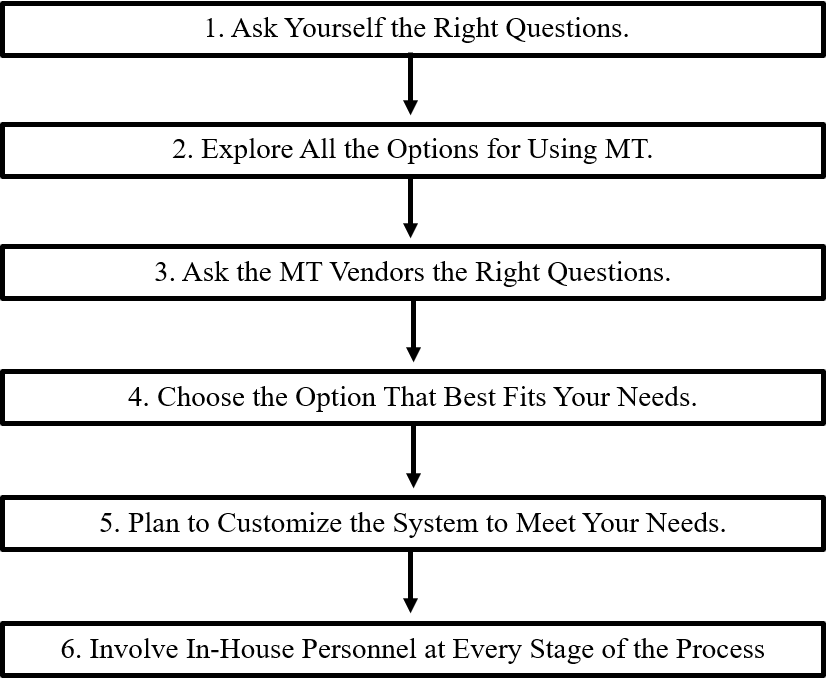
\includegraphics[width=0.8\linewidth]{Fig1.png}
    \caption{Six steps to developing realistic expectations}
    \source{\cite{ryan_machine_1993}}
    \label{fig1}
\end{figure}

As \posscites{ryan_machine_1993} model mainly focuses on matching the client’s expectations with the realistic features of MT, only step three of the model was adapted. Out of the 13 items, nine relevant items were adapted to explore the realistic features of the translation applications, while the remaining four (integration into user environment, training, pre-editing and new releases) were excluded as they were irrelevant to the translation application users’ expectations. For RQ1, the inductive approach was adopted in analysing translation application users’ reviews. The reviews were categorized into themes and subthemes based on the users’ preferences and needs, problems encountered and suggestions to improve the applications using \posscites{kurz_conference_2002} elements of users’ quality expectations. Though the ratings were collected for each user review, they were less informative. Subsequently, a between-app analysis was performed. While for RQ2, the third step of \posscites{ryan_machine_1993} model was adapted to analyze the developers’ description of translation application realistic features. Thereafter, based on the analysis of RQ1 and RQ2, user reviews and developers’ descriptions, the realistic features were compared to indicate the similarities and differences.

\subsection{Materials}\label{sec-autores}
Based on the recommendations from iOS favourites, various blog articles and YouTube videos, the 12 most popular translation applications were purposively selected: \textit{iTranslate, Google Translate}, \textit{Microsoft Translator}, \textit{Naver Papago-AI Translator}, \textit{Easy Language Translator}, \textit{SayHi Translate}, \textit{Speak \& Translate-Translator}, \textit{TextGrabber}, \textit{PONS Online Translator}, \textit{Dear Translate-free English translation}, \textit{iTranslate Converse}, and \textit{Translate -Translator AI}. Among the top five recommendations suggested by Google, \textit{TripLingo} was not included in this study as the user reviews had been removed from the platform. The 12 applications were chosen and at least 20 user reviews posted between September and December 2019 were filtered. Six out of these 12 applications were offered in both \textit{Google Play Store} and \textit{Apple App Store}, whereas three were only available on Google Play Store and three were only on \textit{Apple App Store}. The rating for the \textit{Android} version ranged from 3.7 to 4.6 out of five, whereas the rating for the iOS version ranged from 4.1 to 4.7 out of five. The \textit{Android} version had productivity, tools, education, as well as books and references in the \textit{Google Play Store}.

On the other hand, the iOS version had \textit{videlicet} productivity, reference, business, travel, and utility features. Overall, 240 user reviews from 120 Android users (coded as PS) and 120 Apple users (coded as AS). In addressing RQ2, developers’ descriptions of the applications were extracted from either the application’s official website or the e-store, provided by the developers. Hence, their self-portrayal would suggest the highlight and emphasis of their applications.

\subsection{Data collection and analysis procedure}\label{sec-idioma}
The data was collected in seven steps. User reviews were collected and later classified according to their themes: preferences and needs, problems and improvement suggestions, and categories like accuracy, speed, and availability. Then, a profile of translation application users’ quality expectations was outlined, building a distinct profile, which illustrates the list or collection of quality data summarizing user expectations. Moreover, realistic features were interpreted based on the developers’ description of the translation application using the third step of \posscites{ryan_machine_1993} model. Therefore, “features of the application”, “hardware requirements”, “services offered”, “operational language pairs”, “cost”, “system dictionaries”, “user-specific dictionaries”, “customer support”, “pre-editing”, and “references” were explored in the present study. Features of the application consisted of “favorite”, “history”, and “auto language detection”. Hardware requirements address the type of operating system of applications and the memory storage required for installation or download. Services offered refers to types of translation services and other additional services. Cost refers to the amount needed to pay for the translation service. Some of the applications available in the two e-stores were free, some were paid, and some were free to download but had in-app charges based on the type of translation services. System dictionaries are the general dictionary offered by translation applications. The size, field, and type of entries were the factors that promoted the best coverage for the users. On contrary, user-specific dictionaries considered users’ input into the terminology or expression list for better translation. Customer support tackled the type of assistance provided by the translation application developer when users offered feedback or requested specific improvements. The medium of accepting feedback also reflected the extent the applications were user-friendly. References were the individuals or institutions that used the translation application \cite{ryan_machine_1993}. Thereafter, based on the profile of users’ quality expectations and the realistic features of translation applications, users’ expectations and realistic features were customised to explore and disclose the similarities and differences. Positive and negative reviews were selected to have a fair comparison in identifying users’ needs and preferences as well as the problems encountered. This process is critical to avoid any bias. The names used to indicate translation application users were kept anonymous and confidential.

\section{Results}\label{sec-resumo}
\subsection{Analysis of users’ expectations from translation applications}
The findings uncovered 16 themes for users’ preferences and needs, 14 themes for problems faced by the users, and 12 themes for users’ suggestions to improve the quality of translation applications to enhance user experience.

\subsubsection{Analysis of users’ preferences and needs}\label{sec-secoes}
An examination of the corpus of 240 user reviews from the 12 translation applications available on Google Play Store and Apple App Store revealed a list of 418 users’ preferences or needs. These 418 users’ preferences or needs were merged into 16 themes (\Cref{fig2}, \Cref{tbl1}).

\begin{figure}[h!]
    \centering
    
\includegraphics[width=\linewidth]{Fig2.png}
    \caption{Identify users’ preferences and needs towards translation applications.}
    \source{Own elaboration.}
    \label{fig2}
\end{figure}



\begin{longtable}{p{1cm} p{2.5cm} p{4.5cm} p{5cm}}
\caption{Identify users’ preferences and needs towards translation applications.}
\label{tbl1}
\footnotesize
\\
\toprule
No. & Themes & Categories & Subcategories \\ 
\midrule
\multirow{9}{=}{I} & \multirow{3}{=}{Practicality} & \multirow{4}{=}{Serve travel purpose} & To practice a language \\
& & & To gain information \\
& & & To be appreciated by the locals \\
& & & To fulfill daily translation needs \\
\cmidrule{3-4}
& & \multirow{2}{=}{Serve work purposes in various fields} & Application in general fields \\
& & & Application in specific fields: medical, education and law \\
\cmidrule{3-4}
& & Serve study purposes & \cellcolor[HTML]{EFEFEF} \\
&  & Serve entertainment purposes & \cellcolor[HTML]{EFEFEF} \\
& & Facilitate conversation among family, friends, and helpers & \cellcolor[HTML]{EFEFEF} \\
\midrule
\multirow{8}{=}{II} & \multirow{8}{=}{Functionality} & \multirow{3}{=}{Image translation} & Scan to translate \\
& & & Capture picture to translate \\
& & & Choose an image from the photo gallery \\
\cmidrule{3-4}
& & Voice translation & \cellcolor[HTML]{EFEFEF} \\
\cmidrule{3-4}
& & Conversation translation & \cellcolor[HTML]{EFEFEF} \\
\cmidrule{3-4}
& & Text translation & \cellcolor[HTML]{EFEFEF} \\
\cmidrule{3-4}
& & Website translation & \cellcolor[HTML]{EFEFEF} \\
\cmidrule{3-4}
& & The overall functionality of the app & \cellcolor[HTML]{EFEFEF} \\
\midrule
III & Accuracy & \cellcolor[HTML]{EFEFEF} & \cellcolor[HTML]{EFEFEF} \\
\midrule
\multirow{5}{=}{IV} & \multirow{5}{=}{User-friendliness} & Fullscreen & \cellcolor[HTML]{EFEFEF} \\
\cmidrule{3-4}
& & Language swap & \cellcolor[HTML]{EFEFEF} \\
\cmidrule{3-4}
& & Simple user interface & \cellcolor[HTML]{EFEFEF} \\
\cmidrule{3-4}
& & Themes & \cellcolor[HTML]{EFEFEF} \\ 
\cmidrule{3-4}
& & Landscape mode & \cellcolor[HTML]{EFEFEF} \\ 
\midrule
\multirow{5}{=}{V} & \multirow{4}{=}{Language learning tool} & \multirow{2}{=}{Learn new languages} & Learn new vocabulary and terminology \\
& & & Learn common phrases \\
\cmidrule{3-4}
& & Improve on first language skill & \cellcolor[HTML]{EFEFEF} \\
\cmidrule{3-4}
& & Maintain a second language skill & \cellcolor[HTML]{EFEFEF} \\
\midrule
VI & Variety of languages & \cellcolor[HTML]{EFEFEF} & \cellcolor[HTML]{EFEFEF} \\
\midrule
VII & Speed & \cellcolor[HTML]{EFEFEF} & \cellcolor[HTML]{EFEFEF} \\
\midrule
\multirow{3}{=}{VIII} & \multirow{3}{=}{Cost} & Free app & \cellcolor[HTML]{EFEFEF} \\
\cmidrule{3-4}
& & Paid app & \cellcolor[HTML]{EFEFEF} \\
\cmidrule{3-4}
& & Transparent pricing or subscription plan & \cellcolor[HTML]{EFEFEF} \\
\midrule
 &  & Share to translate feature & \cellcolor[HTML]{EFEFEF} \\
\cmidrule{3-4}
\multirow{6}{=}{IX} & \multirow{6}{=}{Features} & Slide over feature & \cellcolor[HTML]{EFEFEF} \\
\cmidrule{3-4}
& & Save feature & \cellcolor[HTML]{EFEFEF} \\
\cmidrule{3-4}
& & Auto-language detection feature & \cellcolor[HTML]{EFEFEF} \\
\cmidrule{3-4}
& & Pre-translating feature for image translation & \cellcolor[HTML]{EFEFEF} \\
\cmidrule{3-4}
& & The icon that appears when text is copied & \cellcolor[HTML]{EFEFEF} \\
\cmidrule{3-4}
& & Dictation files & \cellcolor[HTML]{EFEFEF} \\
\midrule
X & Availability & \cellcolor[HTML]{EFEFEF} & \cellcolor[HTML]{EFEFEF} \\
\midrule
XI & \multirow{2}{=}{Operationality of language} & Language & \cellcolor[HTML]{EFEFEF} \\
\cmidrule{3-4}
& & Accent and pronunciation & \cellcolor[HTML]{EFEFEF} \\
\midrule
XII & Compatibility & \cellcolor[HTML]{EFEFEF} & \cellcolor[HTML]{EFEFEF} \\
\midrule
XIII & Clarity & \cellcolor[HTML]{EFEFEF} & \cellcolor[HTML]{EFEFEF} \\
\midrule
XIV & Being up to date & \cellcolor[HTML]{EFEFEF} & \cellcolor[HTML]{EFEFEF} \\
\midrule
XV & Application Size & \cellcolor[HTML]{EFEFEF} & \cellcolor[HTML]{EFEFEF} \\
\midrule
XVI & Downloading platform & \cellcolor[HTML]{EFEFEF} & \cellcolor[HTML]{EFEFEF} \\
\bottomrule
\source{Own elaboration.}
\end{longtable}


\subsubsection{Analysis of the types of problems faced by the users}\label{sec-format-simple}
Through a between-app analysis, the sample unveiled a list of 163 problems, which the users came across. These 163 problems were classified into 14 types of problems.

\subsubsection{Mistranslation}\label{sec-links}

\textcite[p. 3]{koponen_assessing_2010} associated the term fidelity with accuracy and mentioned that translation errors related to accuracy occur when the “semantic component” is not “shared by source text and target text”. These errors are labelled as mistranslation in this study. Three factors that caused mistranslation were learned from the 38 user reviews reported on this theme; the inaccuracy of meaning, inconsistent translation, and technical problems (\Cref{fig3}, \Cref{tbl2}).

\begin{figure}[h!]
    \centering
    
\includegraphics[width=\linewidth]{Fig3.png}
    \caption{Identify type of problems faced by users while using the translation applications.}
    \label{fig3}
    \source{Own elaboration.}
\end{figure}


\begin{longtable}{p{1cm} p{2.5cm} p{4.5cm} p{5cm}}
\caption{Identify problems faced by translation application users.}
\label{tbl2}
\footnotesize
\\
\toprule
No. & Themes & Categories & Subcategories \\ 
\midrule
\multirow{6}{=}{I} & \multirow{6}{=}{Mistranslation} & \multirow{3}{=}{Inaccuracy of meaning} & Does not share semantic components \\
& & & Does not share pragmatic equivalence \\
& & & Linguistic inappropriateness of the translation results \\
\cmidrule{3-4}
& & Inconsistent translation & \cellcolor[HTML]{EFEFEF} \\
\cmidrule{3-4}
& & Technical problems & \cellcolor[HTML]{EFEFEF} \\
\cmidrule{3-4}
& & Does not translate at all & \cellcolor[HTML]{EFEFEF} \\
\midrule
\multirow{11}{=}{II} & \multirow{11}{=}{Technical problems} & \multirow{3}{=}{Crash} & When the user enters text \\
& & & When users open the app \\
& & & After the operating system updated \\
\cmidrule{3-4}
& & \multirow{2}{=}{Erroneous behaviour} & Sound system malfunctioned \\
& & & Application became disruptive \\
\cmidrule{3-4}
& & \multirow{6}{=}{Performance issues} & The text recognition feature malfunctioned \\
& & & Translated only part of the text \\
& & & Not recognizing female voices \\
& & & Issues with voice recording feature related to background noises \\
& & & Voice changed randomly \\
& & & The offline language pack malfunctioned \\
\midrule
\multirow{9}{=}{III} & \multirow{9}{=}{Lack of the services offered} & \multirow{3}{=}{Lack of image translation service} & The camera screen could not be zoomed in to enlarge the image \\
& & & Problems relating to the pre-editing and post-editing process \\
& & & Unorganised images \\
\cmidrule{3-4}
& & \multirow{3}{=}{Lack of voice and conversation translation service} & The short duration of the audio recording \\
& & & Did not work with the existence of speech impediment \\
& & & Speech-to-text translation was not available \\
\cmidrule{3-4}
& & \multirow{3}{=}{Lack of text translation service} & Could not translate long paragraphs at a time \\
& & & Text needed to be reinserted \\
& & & No copy option \\
\cmidrule{3-4}
& & The use of two applications to achieve a high success rate & \cellcolor[HTML]{EFEFEF} \\
\cmidrule{3-4}
& & Inaccurate transliteration & \cellcolor[HTML]{EFEFEF} \\
\cmidrule{3-4}
& & Lack in the dictionary service & \cellcolor[HTML]{EFEFEF} \\
\cmidrule{3-4}
& & Lack of offline service & \cellcolor[HTML]{EFEFEF} \\
\cmidrule{3-4}
& & \multirow{2}{=}{Lack in the history or favorite feature} & The favourite feature was old-fashioned \\
& & & Lack of the backup function \\
\midrule
\multirow{3}{=}{IV} & \multirow{3}{=}{Subscription issues} & Issues with subscription pop-ups & \cellcolor[HTML]{EFEFEF} \\
& & Unclear subscription plan & \cellcolor[HTML]{EFEFEF} \\
& & The subscription could not be cancelled & \cellcolor[HTML]{EFEFEF} \\
\midrule
\multirow{3}{=}{V} & \multirow{3}{=}{Pricing issues} & Unreasonable price or unworthy subscription & \cellcolor[HTML]{EFEFEF} \\
& & Stated free but required to pay & \cellcolor[HTML]{EFEFEF} \\
& & Services not offered for free & \cellcolor[HTML]{EFEFEF} \\
\midrule
VI & Lack of language variety & \cellcolor[HTML]{EFEFEF} & \cellcolor[HTML]{EFEFEF} \\
\midrule
\multirow{2}{=}{VII} & \multirow{2}{=}{Not user friendly} & The Voice projection was too fast & \cellcolor[HTML]{EFEFEF} \\ 
\cmidrule{3-4}
& & No tutorial or instructions & \cellcolor[HTML]{EFEFEF} \\
\midrule
X & Availability & The language bar is not visible to change the language & \cellcolor[HTML]{EFEFEF} \\
\midrule
VIII & Not available offline & \cellcolor[HTML]{EFEFEF} & \cellcolor[HTML]{EFEFEF} \\
\midrule
IX & Language not operational & \cellcolor[HTML]{EFEFEF} & \cellcolor[HTML]{EFEFEF} \\
\midrule
X & Slow speed  & \cellcolor[HTML]{EFEFEF} & \cellcolor[HTML]{EFEFEF} \\
\midrule
XI & Not compatible & \cellcolor[HTML]{EFEFEF} & \cellcolor[HTML]{EFEFEF} \\
\midrule
XII & Poor customer support & \cellcolor[HTML]{EFEFEF} & \cellcolor[HTML]{EFEFEF} \\
\midrule
XIII & Advertisement issues & \cellcolor[HTML]{EFEFEF} & \cellcolor[HTML]{EFEFEF} \\
\midrule
XIV & Negative modification & \cellcolor[HTML]{EFEFEF} & \cellcolor[HTML]{EFEFEF} \\
\bottomrule
\source{Own elaboration.}
\end{longtable}



\subsubsection{Analysis of users’ suggestions to improve the quality of translation applications}\label{sec-outras-estr}
From the 240 user reviews, 120 suggestions and 11 themes were identified; improving the existing services (29.17\%), adding more languages (18.33\%), fixing the technical problems (12.5\%), continuing with adding new features (10.83\%), improving the accuracy of the translation (7.5\%), offering offline services (5.83\%), improving the operationality of languages (5\%), repricing, reconstructing subscription plan or making services free (4.17\%), reverting to the old version (2.5\%), improving the speed (2.5\%), and improving on the user interface of applications (1.67\%) (\Cref{fig4}, \Cref{tbl3}).

\begin{figure}[h!]
    \centering
    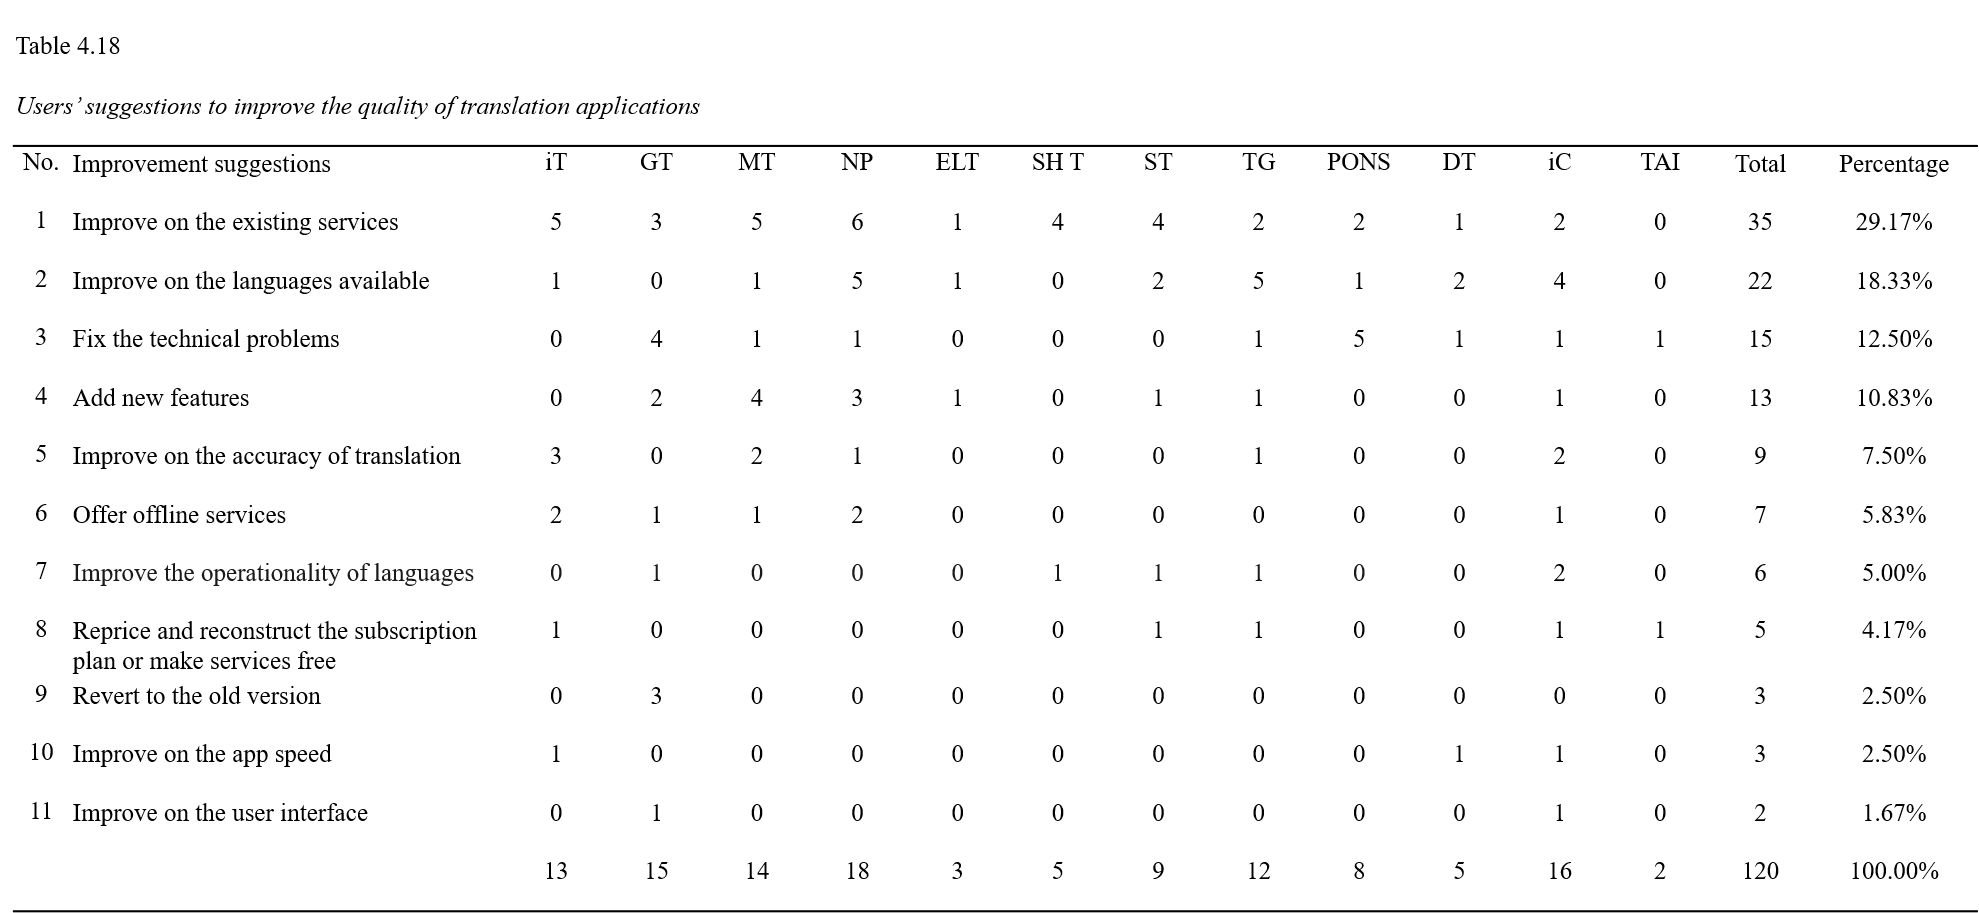
\includegraphics[width=\linewidth]{Fig4.png}
    \caption{Identify user’s suggestions to improve the quality of translation applications}
    \source{Own elaboration}
    \label{fig4}
\end{figure}




\begin{longtable}{p{1cm} p{2.5cm} p{4.5cm} p{5cm}}
\caption{Improvement suggestions proposed by the translation application users.}
\label{tbl3}
\footnotesize
\\
\toprule
No. & Themes & Categories & Subcategories \\ 
\midrule
\multirow{5}{=}{I} & \multirow{5}{=}{Improve on the existing services} & \multirow{3}{=}{Improve the image translation service} & Allow users to check the recognised text before translating \\
& & & Allow scan and translate function \\
& & & Allow users to add text to the image \\
\cmidrule{3-4}
& & \multirow{2}{=}{Improve the voice translation service} & Increase voice recording duration \\
& & & Improve the auto-language detection function \\
\midrule
\multirow{6}{=}{II} & \multirow{6}{=}{Improve on the existing services} & \multirow{2}{=}{Improve the conversation translation service} & Allow users to control the voice recording duration for conversation mode \\
& & & Allow the conversation mode to type instead of just voice recognition \\
\cmidrule{3-4}
& & Improve the text translation service & \cellcolor[HTML]{EFEFEF} \\
\cmidrule{3-4}
& & Improve the website translation service & \cellcolor[HTML]{EFEFEF} \\
\cmidrule{3-4}
& & \multirow{2}{=}{Improve the dictionary service} & Include meanings of words and the sentence examples \\
& & & Add the pronunciation of words \\
\midrule
\multirow{3}{=}{III} & \multirow{3}{=}{Improve on the languages available} & Add more languages & \cellcolor[HTML]{EFEFEF} \\
\cmidrule{3-4}
& & Add more types of writing system & \cellcolor[HTML]{EFEFEF} \\
\cmidrule{3-4}
& & Add informal or casual language & \cellcolor[HTML]{EFEFEF} \\
\midrule
IV & Fix the technical problems & \cellcolor[HTML]{EFEFEF} & \cellcolor[HTML]{EFEFEF} \\
\midrule
\multirow{7}{=}{V} & \multirow{7}{=}{Add new features} & Translation services extension to other mobile applications & \cellcolor[HTML]{EFEFEF} \\
\cmidrule{3-4}
& & Landscape mode & \cellcolor[HTML]{EFEFEF} \\
\cmidrule{3-4}
& & Copy feature & \cellcolor[HTML]{EFEFEF} \\
\cmidrule{3-4}
& & Page numbering feature & \cellcolor[HTML]{EFEFEF} \\
\cmidrule{3-4}
& & Contact feature for conversation translation & \cellcolor[HTML]{EFEFEF} \\
\cmidrule{3-4}
& & Memory flashcards to aid language learning & \cellcolor[HTML]{EFEFEF} \\
\cmidrule{3-4}
& & Artificial Intelligence (AI) technology & \cellcolor[HTML]{EFEFEF} \\
\midrule
VI & Improve the accuracy of the translation & \cellcolor[HTML]{EFEFEF} & \cellcolor[HTML]{EFEFEF} \\
\midrule
VII & Offer offline services & \cellcolor[HTML]{EFEFEF} & \cellcolor[HTML]{EFEFEF} \\
\midrule
VIII & Improve the operationality of languages & \cellcolor[HTML]{EFEFEF} & \cellcolor[HTML]{EFEFEF} \\
\midrule
IX & Reprice and reconstruct the subscription plan or make services free & \cellcolor[HTML]{EFEFEF} & \cellcolor[HTML]{EFEFEF} \\
\midrule
X & Revert to the old version & \cellcolor[HTML]{EFEFEF} & \cellcolor[HTML]{EFEFEF} \\
\midrule
XI & Improve the application speed & \cellcolor[HTML]{EFEFEF} & \cellcolor[HTML]{EFEFEF} \\
\midrule
XII & Improve the user interface & \cellcolor[HTML]{EFEFEF} & \cellcolor[HTML]{EFEFEF} \\
\bottomrule
\source{Own elaboration.}
\end{longtable}

\subsection{Analysis of self-portrayal description of translation application developers on their product}\label{sec-listas}
Adapted from \posscites{ryan_machine_1993} paper on matching realistic features of MT to client’s expectations, the product description, and the realistic features of the 12 applications by the developers were explored. The findings uncovered nine themes specified by the developers: the features of translation applications, services offered, hardware requirements, operational language pairs, cost, system dictionaries, user-specific dictionaries, customer support, and references.

\subsubsection{Application features}\label{sec-figuras-tabelas}
The following were the features available on the 12 applications.

\begin{enumerate}
    \item \textbf{Slide over and split view} \\
    Based on the self-portrayal translation application description, the slide-over and split view feature was only available on \textit{iTranslate}. Slide over feature allows users to work on several applications synchronously while the split view feature enables users to view two applications at a time.
    \item \textbf{Auto language detection} \\
    Using the auto language detection feature, the application recognises the SL automatically without having to choose the language manually by the users. This feature was highlighted in \textit{iTranslate}, \textit{Speak \& Translate-Translator}, and \textit{iTranslate Converse} to activate the “detect language” option if users do not know the language of the ST.
    \item \textbf{Translation services extension} \\
    Translation services extension refers to the use of translation services on other mobile applications. Users can perform the translation in any application such as messaging applications. For example, users can translate text messages while chatting, without having to copy the text and paste it into the translation application.  Google Translate has a “tap to translate” feature, whereby the translation will pop up whenever a text is copied. This feature is called \textit{Papago Mini} in \textit{Naver Papago-AI Translator}.
    \item \textbf{Availability} \\
    All 12 applications were available for online usage. Five of them offered offline mode, and three allowed offline usage if the users downloaded the language pack beforehand. Some, like the \textit{Easy Language Translator} and \textit{SayHi Translate}, required an internet connection to function.
\end{enumerate}
    
\begin{enumerate}[label=\alph*.]
    \item \textit{Offline mode} \\
    The feature does not apply to all types of translation services. While \textit{Google Translate}, \textit{TextGrabber Scan and Translate}, and \textit{Dear Translate-free English Translation} delivered offline services free, some like \textit{Speak \& Translate-Translator} offered offline mode under in-app purchase. The offline mode for text translation catered for a lesser number of languages compared to the online mode.
    \item \textit{Pre-downloaded language pack or dictionary} \\
    Some applications like \textit{PONS Online Translator} did not offer offline mode, but they allow users to download the language pack or dictionary for offline use when the users travel without an internet connection. The offline language pack required additional storage space.
\end{enumerate}

\begin{enumerate}
    \item \textbf{Accuracy} \\
    Accuracy of translation was highlighted in some applications like \textit{SayHi Translate}: “Say what you want, we’ll transcribe it quickly and accurately” and “Superior Translation Accuracy”.
    \item \textbf{History and favourite} \\
    With this feature, users can also edit and merge all the captured texts in the note list. In \textit{TextGrabber Scan and Translate}, “users will never lose the previously recognised and translated texts” and QR codes, as all results are retrievable. \textit{Speak \& Translate-Translator} has an iCloud integration, in which the history is synchronised across all users’ Apple devices. In \textit{PONS Online Translator}, users can find their most recent searches. The phrasebook in \textit{Google Translate} enables users to star, pin and save the translated words and phrases for future reference. \textit{Easy Language Translator} can save voice translation as MP3.
    \item \textbf{Copy and share} \\
  \textit{  iTranslate, Google Translate, Microsoft Translator, Easy Language Translator, SayHi Translate, TextGrabber Scan} and Translate, and PONS Online Translator had a copy and share features via the system sharing. For instance, \textit{SayHi Translate} can share conversations via email, SMS, Facebook and Twitter.
    \item \textbf{Allow location} \\
    \textit{Naver Papago-AI Translator and Speak \& Translate-Translator} claimed that by allowing location, the translation service would be “better” because it enables the automatic language selection for the host country, especially when users travel.
    \item \textbf{Fast speed} \\
    Speed is an essential feature for translation applications. The 12 applications explicitly or implicitly stated this feature by using terms like “fast”, “fastest”, “quick”, “instant”, “blazing fast”, and “real-time”.
    \item \textbf{User-friendly interface} \\
    A user-friendly interface refers to an application interface that is easy to use and navigate. For example, \textit{SayHi Translate} and \textit{iTranslate Converse} were promoted as “simple and modern”, and “simple and easy” respectively.
    \item \textbf{Display text as a big sign} \\
    This feature allows users to adjust font sizes and audio prompts to assist visually impaired people. \textit{TextGrabber Scan and Translate} can copy the text to the clipboard for the text-to-speech applications to read aloud anything on the screen. \textit{PONS Online Translator} uses the zoom function.
    \item \textbf{Advertisement-free} \\
    Most of the free applications have advertisements that pop up while using the app. Some like \textit{PONS Online Translator} claim to be entirely ad-free, and some like \textit{Speak \& Translate-Translator} need a subscription to its premium plan to enjoy ads-free translation.
    \item \textbf{Transliteration} \\
    The transliteration feature is introduced as a pronunciation guide for the users. Replacing characters or words with equivalent phonetics, helps users to pronounce the translation. \textit{iTranslate and Microsoft Translator} had this feature. \textit{Microsoft Translator} included Pinyin (the romanization of Chinese characters) for the Chinese language.
    \item \textbf{Example sentences} \\
    In assisting users to identify the most accurate translation, some applications like \textit{PONS Online Translator} provided example sentences for the users as “language in context” helps users to find the correct information.
    \item \textbf{Full transcript of the conversation} \\
    This feature enables users to keep a copy of the conversation translation for future reference. For example, \textit{iTranslate Converse} allows users to view and export full transcripts for every voice conversation.
    \item \textbf{Global conversation} \\
    With this feature, users can carry out a conversation with people who speak a different language by using the expressions listed. For example, \textit{Naver Papago-AI Translator} consists of basic expressions that are available even without a network connection.
\end{enumerate}

\subsubsection{Services offered}\label{sec-quotesandfootnotes}
Six major types of services were identified, while five of them were related to translation services.

\begin{enumerate}
    \item \textbf{Text translation} \\
    Among the nine applications of text translation, only \textit{Google Translate} and \textit{Naver Papago-AI} had a videlicet typing and/or drawing text feature by which users draw or handwrite text characters with fingers. The translation mode varied in the applications, i.e. text-to-text or text-to-speech, though the text-to-speech mode is not available in most of them. \textit{iTranslate} allows users to choose either male or female voices as the output voice. The number of supported languages can differ between online and offline modes. For instance, iTranslate supports over 100 languages online and as less as 38 languages offline. For this feature, \textit{Microsoft Translator} initiated a function whereby users can look up alternate translations to find the best translation if the application itself can find any result from its system dictionary.
    \item \textbf{Voice translation} \\
    With the voice recognition feature, the applications require users to allow the microphone to recognise the users’ voices. It converts the speech to text and translates them into another language. \textit{iTranslate}, \textit{Google Translate}, \textit{Microsoft Translator}, \textit{Naver Papago-AI Translator}, \textit{Easy Language Translator}, \textit{SayHi Translate}, \textit{Speak \& Translate - Translator}, \textit{Dear Translate-free English Translation}, and \textit{Translate-Translator AI} performed instant voice translations. Some applications allowed users to control the speed of voice output, including \textit{SayHi Translate} and \textit{Speak \& Translate-Translator}. Users could adjust the speed of voice in the voice setting. The speech-to-text mode was also available in \textit{Naver Papago-AI Translator}, \textit{Easy Language Translator}, and \textit{Speak \& Translate-Translator}.
    \item \textbf{Conversation translation} \\
    Like voice translation, conversation translation stands out for its ability to allow users to simultaneously speak in each other’s language when talking one-on-one. For example, \textit{Microsoft Translator} has a split-screen mode for two participants to have a real-time bilingual and multilingual conversation. \textit{iTranslate Converse} emphasised its specialty in working well in a noisy environment.
    \item \textbf{Image translation} \\
    When users allow the applications to access the camera and/or the photo gallery, image translation can be carried out in three ways: videlicet scan to translate, take a photo to translate or upload an existing photo to translate. In \textit{Translate-Translator AI} and innovative OCR technology in \textit{TextGrabber Scan and Translate}, the text is identified in the image instantly and is simultaneously translated. This service is very beneficial in live stream video, television or smartphone screens, receipts, menus and signs, labels and counters, travel documents, magazine articles and book fragments, manuals and instructions, and recipe ingredients. \textit{TextGrabber Scan and Translate} also enables users to listen to the recognised text, using \textit{VoiceOver} or using the Speech option.
    \item \textbf{Website translation} \\
  \textit{  iTranslate, Naver Papago-AI Translator}, and \textit{Dear Translate-free English Translation} had this feature. For example, iTranslate performed website translations in over 40 languages.
    \item \textbf{Emotion translation} \\
    Offered only in \textit{Dear Translate-free English Translation}, emotion translation is intended to “add taste” to the text.
    \item \textbf{Other services} \\
    Other than the five types of translation services offered, the following services were offered in the applications:
    \begin{enumerate}[label=\alph*.]
        \item Dictionary
        \item Phrasebook
        \item QR code reader
    \end{enumerate}
\end{enumerate}

\subsubsection{Hardware requirements}\label{sec-equacao}
The hardware requirements for a translation application include the operating system version of the device and the available storage space. The variety of devices that are compatible with these applications is controlled between devices with the android operating system and the iOS operating system. Taking Apple products as an example, most of the applications required iOS 9.0 and Android 4.2 versions and above to install these applications, though it varied with the device.

\subsubsection{Operational language pairs}\label{sec-codigos}
Without mentioning how operational the language pairs are, the developers highlighted the number of languages. Most of the applications support over 100 languages. For instance, \textit{Speak \& Translate-Translator} supported 117 languages for text translations and 54 languages for voice translations. Those which supported less than 100 languages were Microsoft Translator (60 languages), Naver Papago-AI Translator (13), SayHi Translate (15), iTranslate Converse (38), and PONS Online Translator (36).


\subsubsection{Cost}\label{sec-contributors-expl}
\textit{Google Translate}, \textit{Microsoft Translator}, \textit{Naver Papago-AI Translator}, \textit{Easy Language Translator}, \textit{SayHi Translate}, and \textit{Dear Translate-free English Translation} were free. Some free applications like \textit{Speak \& Translate-Translator} had a limited number of free daily translations. The rate ranged from $ to about $80 per year, though some applications offer a pay-once-and-use-for-life subscription, like \textit{TextGrabber Scan and Translate}.

\subsubsection{System dictionaries}\label{sec-contributors-expl}
Most developers did not mention the type of system dictionaries used in developing the applications. Based on their target users, the system dictionary employs the general dictionary with glossaries that cater to general usage instead of specific subject fields. \textit{Google Translation} has upgraded from phrase-based MT (PBMT) to the neural machine translation system (NMT). NMT translates whole sentences at a time, rather than part-by-part. In other words, the system looks at the bigger picture of the ST to help determine the most appropriate choice of words for the translation, followed by adjusting the syntax of the sentence to improve the translation quality. Consequently, a more natural translation can be generated. \textit{Microsoft Translator} uses a cloud-based MT system. \textit{TextGrabber Scan and Translate} claimed that the translation is performed by a third-party service, and \textit{PONS Online Translator} affirmed that their translations are of editorially reviewed quality.

\subsubsection{User-specific dictionaries}\label{sec-contributors-expl}
Applications with user-specific dictionaries collect users’ input to enhance the accuracy of the translation. For example, \textit{Google Translate} enables users’ input through the fill-in-the-blank or multiple-choice questions. As the users proceed to the next level, they will be asked to suggest translations and validate others’ translations.

\subsubsection{Customer support}\label{sec-contributors-expl}
All 12 applications clearly stated the way to connect to customer support in the e-stores for any queries, feedback, or app-related issues. The users could either visit their official website or contact them via the link or email address provided.

\subsubsection{References}\label{sec-contributors-expl}
According to \textcite{ryan_machine_1993}, references are those people that the users can refer to when making decisions. As most of the translation application target users are travellers, students, and business professionals as stated in five of the 12 selected applications, the users can refer to the endorsement by credible individuals or institutions (\Cref{tbl4}).





\begin{longtable}{p{1cm} p{2.5cm} p{4.5cm} p{5cm}}
\caption{Self-portrayal description by the translation application developers.}
\label{tbl4}
\footnotesize
\\
\toprule
No. & Themes & Categories & Subcategories \\ 
\midrule
\multirow{17}{=}{I} & \multirow{17}{=}{Application features} & Slide over and split view & \cellcolor[HTML]{EFEFEF} \\
\cmidrule{3-4}
& & Auto language detection & \cellcolor[HTML]{EFEFEF} \\
\cmidrule{3-4}
& & Translation services extension & \cellcolor[HTML]{EFEFEF} \\
\cmidrule{3-4}
& & \multirow{2}{=}{Availability} & Offline mode \\
& & & Pre downloaded language pack or dictionary \\
\cmidrule{3-4}
& & Accuracy & \cellcolor[HTML]{EFEFEF} \\
\cmidrule{3-4}
& & History and favorites & \cellcolor[HTML]{EFEFEF} \\
\cmidrule{3-4}
& & Copy and share & \cellcolor[HTML]{EFEFEF} \\
\cmidrule{3-4}
& & Allow location & \cellcolor[HTML]{EFEFEF} \\
\cmidrule{3-4}
& & Fast speed & \cellcolor[HTML]{EFEFEF} \\
\cmidrule{3-4}
& & User-friendly interface & \cellcolor[HTML]{EFEFEF} \\
\cmidrule{3-4}
& & Display text as a big sign & \cellcolor[HTML]{EFEFEF} \\
\cmidrule{3-4}
& & Advertisement-free & \cellcolor[HTML]{EFEFEF} \\
\cmidrule{3-4}
& & Transliteration & \cellcolor[HTML]{EFEFEF} \\
\cmidrule{3-4}
& & Example sentences & \cellcolor[HTML]{EFEFEF} \\
\cmidrule{3-4}
& & Full transcript of the conversation & \cellcolor[HTML]{EFEFEF} \\
\cmidrule{3-4}
& & Global conversation & \cellcolor[HTML]{EFEFEF} \\
\midrule
\multirow{9}{=}{II} & Text translation & \cellcolor[HTML]{EFEFEF} \\
\cmidrule{3-4}
& & Voice translation & \cellcolor[HTML]{EFEFEF} \\
\cmidrule{3-4}
& & Conversation translation & \cellcolor[HTML]{EFEFEF} \\
\cmidrule{3-4}
& & Image translation & \cellcolor[HTML]{EFEFEF} \\
\cmidrule{3-4}
& & Website translation & \cellcolor[HTML]{EFEFEF} \\
\cmidrule{3-4}
& & Emotion translation & \cellcolor[HTML]{EFEFEF} \\
\cmidrule{3-4}
& & \multirow{3}{=}{Other services} & Dictionary \\
& & & Phrasebook \\
& & & QR code reader \\
\midrule
III & \multirow{2}{=}{Hardware requirements} & \multirow{2}{=}{Operating system version} & iOS and watchOS \\
& & & Android \\
\cmidrule{3-4}
& & Storage space & \cellcolor[HTML]{EFEFEF} \\
\midrule
IV & Operational language pairs & \cellcolor[HTML]{EFEFEF} & \cellcolor[HTML]{EFEFEF} \\
\midrule
V & Cost & \cellcolor[HTML]{EFEFEF} & \cellcolor[HTML]{EFEFEF}\\
\midrule
VI & System dictionaries & \cellcolor[HTML]{EFEFEF} & \cellcolor[HTML]{EFEFEF} \\
\midrule
VII & User-specific dictionaries & \cellcolor[HTML]{EFEFEF} & \cellcolor[HTML]{EFEFEF} \\
\midrule
VIII & Customer support & \cellcolor[HTML]{EFEFEF} & \cellcolor[HTML]{EFEFEF} \\
\midrule
IX & References & \cellcolor[HTML]{EFEFEF} & \cellcolor[HTML]{EFEFEF} \\
\bottomrule
\source{Own elaboration.}
\end{longtable}

\subsection{Analysis of users’ expectations about customization of realistic features in translation applications}
Among the 16 preferences and needs, three were related to translation quality while 13 were linked to the service quality of the applications. Other than mistranslations, the remaining 12 problems can be associated with service quality.

\subsubsection{Translation quality}\label{sec-contributors-expl}
Users were concerned about the accuracy and clarity of translation (14.11\%). Mistranslation tops the list of problems (23.31\%), while the eleven types of suggestions related to translation quality consisted of 7.5\% of entire suggestions. When comparing users’ expectations with the realistic features, accuracy was only mentioned explicitly in \textit{SayHi Translate} (“voice translation for everyone”) and \textit{iTranslate Converse} “specialised in conversation translation”.  For \textit{PONS Online Translator} developers, “reliability” was highlighted. \textit{Translate-Translator AI} merely described its translation quality as “best”. The other two aspects that could affect the translation quality are the operationality of languages and the translation application system. The developers highlighted the number and variety of languages offered instead. This created great concern among the users as some users complained that “languages are wrong” and the application “pronounces even the simplest phrases wrong in every language besides English”. Despite the “translation system” being only touched in three of the applications, it is crucial in determining how the SL is translated to the TL (\Cref{tbl5}).

\begin{table}[h!]
\centering
\begin{threeparttable}
\caption{Identify perspectives of Developers and users on translation quality.}
\label{tbl5}
\footnotesize
\begin{tabular}{p{1cm} p{5cm} p{2cm} p{2cm}}
\toprule
No. & Qualities & Developer(s) & User(s) \\ 
\midrule
\multirow{4}{=}{1} & Translation qualities criteria: & & \\
& I. Accuracy & \cmark & \cmark \\
& II. Clarity & \xmark & \cmark \\
& III. Reliability & \cmark & \xmark \\
\midrule
\multirow{3}{=}{2} & Factors that may influence translation qualities: & & \\
& I. Operationality of language & \xmark & \cmark \\
& II. Translation system & \cmark & \xmark \\
\bottomrule
\end{tabular}
\source{Own elaboration.}
\end{threeparttable}
\end{table}

\subsubsection{Service quality}
Among 240 translation application users, service quality made up 85.89\% of the users’ preferences and needs, 76.69\% of the problems, and 92.5\% of the improvement suggestions. On the other hand, evidence of service quality was found in the 12 application descriptions; namely application features, types of services offered, the number of language support, variety of subscription plans, and customer support. In comparing the user reviews with the realistic features of the applications, seven themes were driven in describing the extent to which realistic features of applications are matching with users’ expectations.

\begin{enumerate}
    \item \textbf{Application features} \\
    Most of the features offered in these 12 applications met the users’ expectations, though there were problems encountered by the users. The seven features mentioned in the users’ preferences and needs are covered within the 16 kinds of application features, except the pre-translating feature for image translation. None of the applications possessed all 16 types of features. The greatest number of features belonged to \textit{iTranslate}, which provided eight out of 16, followed by \textit{PONS Online Translator} with seven, and \textit{Google Translate} with six features.
    
	The four features of page numbering feature for image translation, contact feature for conversation translation, memory flashcards to aid language learning, and a more intuitive AI technology was not among those primary features. While 12 applications claimed to provide fast, simultaneous and real-time translation services, 3.07\% of the users pinpointed the slow speed of website translation, offline translation, and translation on the \textit{Apple} watch.
 
	Furthermore, while the backup function of the history and favourite features were claimed to be missing from a good translation app, the lack of the copy and share features led to “disappointment”. Finally, the user-friendliness of the applications comes next, which was downplayed by the developers as only two out of twelve applications promised a simple and easy user interface.
 \item \textbf{Services offered} \\
 Experiencing the five types of translation services offered as promised in these twelve selected applications, users reviewed the practicality, functionality, and availability of these services positively and negatively. In translation applications, practicality looks into the state of applicability in real practice. In terms of practicality, users complimented the usability of the application to serve travel, work, study, entertainment, and daily conversation purposes. These translation services aided the process of learning new languages, improving first language skills, and maintaining second language skills, in addition to breaking down language barriers. Concerning the functionality of the applications, most of the reviews are inclined towards the image translation service. The users experienced an enjoyable image translation process whereby no text typing or voice recording is required for a translation to be performed.

However, several problems were related to the pre-editing and post-editing processes, and text recognition feature malfunction. Voice translation and conversation translation are often linked because both are recognizing and projecting TL mainly verbally. Good voice recognition is deemed necessary to ensure that the input is registered accurately. Also, the brief voice recording duration concerned the users. Another significant problem was related to the length of the text. Many users highlighted the need for text translation services that can translate long paragraphs, or at least long sentences. None of these 12 applications highlighted the above, as checked in the application descriptions. Website translation services were only requested twice in the user reviews, one depicted as negative feedback, and another as positive towards the website translation service offered by the applications. With five applications offering offline services and three with pre-downloaded language packs, the problem of availability persists.
 
While availability takes up 3.11\% of the users’ preferences and needs, it forms 4.29\% of problems faced by the users and 5.83\% of the improvement suggestions. Users wish to have an application that does not require an internet connection so that they can use it anywhere at any time in addition to the online availability. Yet, no solution was suggested by users to resolve this problem.

\item \textbf{Variety of languages} \\
Despite over 100 languages being supported by the seven applications and over 50 languages by two, the users were dissatisfied with the absence of certain languages. The romanization of Japanese, Korean, and Chinese written languages was suggested to be included to aid in the pronunciation of words. Furthermore, the informal and casual forms of languages were encouraged to be added.

\item \textbf{Compatibility} \\
Some applications with Android devices running on the upgraded operating system “stopped working”.

\item \textbf{Cost} \\
Some users were willing to pay if the overall quality, particularly accuracy, is improved. The subscription plan should be worthy of the price and be transparent in terms of features and services covered.

\item \textbf{Customer support} \\
The attitude of customer service personnel was in a few comments called “rude and dishonest”.

\item \textbf{Being up to date} \\
All users’ preferences and needs, problems, and improvement suggestions were to be taken into consideration with the application update in “What’s New” in both e-stores (\Cref{tbl6}).  
\end{enumerate}





\begin{longtable}{p{1cm} p{2.5cm} p{4.5cm} p{5cm}}
\caption{Summary of service quality criteria.}
\label{tbl6}
\footnotesize
\\
\toprule
No. & Themes & Categories & Subcategories \\ 
\midrule
\multirow{5}{=}{I} & \multirow{5}{=}{Application features} & Variety of features & \cellcolor[HTML]{EFEFEF} \\
\cmidrule{3-4}
& & Speed & \cellcolor[HTML]{EFEFEF} \\
\cmidrule{3-4}
& & History and favorite & \cellcolor[HTML]{EFEFEF} \\
\cmidrule{3-4}
& & Copy and share & \cellcolor[HTML]{EFEFEF} \\
\cmidrule{3-4}
& & Simple user interface & \cellcolor[HTML]{EFEFEF} \\
\midrule
\multirow{10}{=}{II} & \multirow{10}{=}{Services offered} & \multirow{2}{=}{Practicality} & Serve users’ needs \\
& & & Aid in language learning \\
\cmidrule{3-4}
& & \multirow{5}{=}{Functionality} & Image translation \\
& & & Voice translation \\
& & & Conversation translation \\
& & & Text translation \\
& & & Website translation \\
\cmidrule{3-4}
& & \multirow{3}{=}{Availability} & Online mode \\
& & & Offline mode \\
& & & Pre downloaded language pack \\
\midrule
\multirow{3}{=}{III} & \multirow{3}{=}{Variety of languages} & Number of languages & \cellcolor[HTML]{EFEFEF} \\
& & Romanization of written language & \cellcolor[HTML]{EFEFEF} \\
& & Informal languages & \cellcolor[HTML]{EFEFEF} \\
\midrule
\multirow{2}{=}{IV} & \multirow{2}{=}{Compatibility} & Android devices & \cellcolor[HTML]{EFEFEF} \\
& & iOS devices & \cellcolor[HTML]{EFEFEF} \\
\midrule
\multirow{2}{=}{V} & \multirow{2}{=}{Cost} & Worthiness \cellcolor[HTML]{EFEFEF} \\
& & Transparency of plan & \cellcolor[HTML]{EFEFEF} \\
\midrule
VI & Customer support & The attitude of the customer service & \cellcolor[HTML]{EFEFEF} \\
\midrule
VII & Being up to date & \cellcolor[HTML]{EFEFEF} & \cellcolor[HTML]{EFEFEF} \\
\bottomrule
\source{Own elaboration.}
\end{longtable}

Translation applications, as the new frontier of MT, are introduced to the market to serve users’ needs for various purposes such as travel, work, and daily conversation with family. To fill in the research gap in users’ expectations and realistic features of the translation applications through a qualitative method, an inductive approach was employed to group 240 user reviews and 12 translation application descriptions into themes and categories.

Consequently, the data were analyzed to the extent the users’ expectations and realistic features are corresponding. The 16 types of users’ preferences and needs, as well as the 14 types of problems, were compiled from the users. The results indicated that there is a lot of room for improvement in translation applications. In understanding users’ expectations towards translation applications, users’ suggestions were divided into 11 themes, which may contribute to developing the translation application users’ expectation profile.

The between-app analysis was conducted on the 12 selected translation application descriptions. Adapted from \posscites{ryan_machine_1993} third step in developing realistic expectations, nine themes of translation application realistic features were explored. While all these translation applications promised instant translation, there were differences in the translation quality and service quality. It can be concluded that a multifunctional translation application is more convenient and time-saving for the users as they would not need to download multiple applications and switch between the translation applications to perform translations of videlicet text, voice, and image.

Comparing the users’ expectations with the realistic features highlighted by the application, a list of translation quality criteria and service quality criteria were outlined. Three translation quality criteria derived from the findings included accuracy, clarity, and reliability whereas the possible factors influencing these qualities were the operationality of languages and the type of translation system. Seven aspects of application features, services offered, variety of languages, compatibility, cost, customer support, and being up to date in the list were explored to identify the extent to which users’ expectations of translation applications were customised with realistic features. The analysis of the findings from users' and the developers’ perspectives revealed a fair comparison of translation quality and service quality for the applications chosen purposively. A guideline for improving translation application could be developed based on these findings.


\section{Discussion and conclusion}\label{sec-conclusao}
Quality begins with customer needs and ends with customer perception. Quality service is delivered when “its/his product/service meets or exceeds customer needs, requirements, and expectations” \cite{kotler_principles_1994}. The findings of the present study confirmed that users emphasise accuracy and clarity and the majority of the users labeled accuracy as “good” translation quality. Consistent with previous research \cite{barnwell_introduction_1980,nababan_teori_2008}, it can be concluded that the users were more ST-oriented, intending to understand the original message. Whereas some who cherished clarity tended to be more TT oriented and more wished to be understood by others, in line with \textcite{chesterman_memes_2000} findings. Therefore, the reliability of the translation results should be examined by the developers.

Mistranslation was a problem that concerned users the most, and most users’ top demand to the translation application developers was in improving the accuracy of the translation. In agreement with \textcite{koponen_assessing_2010} results on mistranslation as the most typical MT error in affecting accuracy, the present findings discovered inequivalence of semantic components and pragmatic components, as well as the inappropriateness of word choice used in the applications. Hence, these problems call for the developers’ attention. The translation application developers are advised to look into the operationality of languages and the translation system they adopted in their applications. Different types of translation systems incorporated in the applications determine how an ST is being translated. A good move was by \textit{Google Translate}, which replaced the former PBMT with NMT for higher accuracy \cite{jean_does_2017}. With these refinements, the users can expect the translation quality of translation applications to improve.

Service quality based on users’ points of view consisted of all factors that guarantee user satisfaction. In the present study, while most of the application features met the users’ expectations, the pre-editing feature for image translation was found essential but absent in the developers’ self-portrayal description of their product. Pre-editing is also regarded by \textcite{ryan_machine_1993} to be considered by the clients in customizing an MT system to their needs. The same applies to the translation applications; the developers could consider including this pre-editing feature under the image translation service. The page numbering feature for image translation, contact feature for conversation translation, and memory flashcards, via the implementation of AI technology were the other important features.

The types of services offered vary across different applications. In terms of practicality, functionality, and availability of the services offered, the findings suggested that users appreciate the applications that serve their purposes, function well, and are available for offline usage. However, the technical problems and malfunctions reported by the users were ranked second in the list, which requires modification by the developers. The variety of language support was highlighted by the developers in the product description. Hence, some problems were related to the absence of certain languages from the language support. Romanization of written characters was also found as a need to aid in the pronunciation of words. Informal languages were expected to be added to the system. This could be due to the users’ wish to speak native-like or to be understood and accepted by others \cite{herman_technical_1993}.

The users did not report system compatibility as a major problem, except for some smartwatches and tablets running on either the iOS or Android operating system. Furthermore, while most users preferred a free application, some were willing to pay if the translation quality and service quality were “worth” the price. Most users complained about the advertisement pop-ups. While the customer support took the initiative to respond, some service attitudes were claimed to have left a negative impression on the users. Time-to-time updates and modifications were acceptable to the users.

The most holistic translation application in terms of features (\textit{iTranslate} with eight features), offered a dictionary in addition to all five major types of translation in both online and offline modes, was compatible with both Android and iOS, providing customer support, and delivered new updates from time to time. This application could be taken as an example of a “good” translation application. However, the only downside of this application from the users’ perspective was that they had to pay for the services or subscribe to the premium plan to experience all the services.

The present study has some empirical and theoretical implications in the scope of translation application development. The findings can be used as a guide for the translation application developers to further improve the translation and service quality of their products based on the users’ preferences and needs, and issues faced by the users. The developers may also investigate the feasibility of the proposed recommendations. The translation application vendors may take the profile of users’ expectations into consideration when marketing the application. In addition, stakeholders and potential investors may refer to the findings to identify the market gap in existing translation applications.

The weaknesses and strengths of each application described in detail in terms of features, services offered, hardware requirements, cost, language support, system dictionaries, user-specific dictionaries, customer support, and references determined the extent users’ expectations were realistically customised so that the users can adjust their expectations from the translation applications considering the descriptions often promise a quality that may not be realistically experienced by the users. Furthermore, this study could also contribute to human translators. Knowing the differences between users’ expectations and realistic features may improve translators’ knowledge in the interdisciplinary field of translation and technology \cite{doherty_translations|_2016}. Finally, the developers can refer to this research as a guide in their future updates to design or update a translation application that values the users’ expectations. Future studies may focus on applications that provide the same variety of translation services. A comparative analysis between translation applications can contribute to the identification of the similarities and differences in the specific niche, looking into whether a multifunctional translation application or a single specialised translation application is better in terms of translation quality and service quality.


\printbibliography\label{sec-bib}
% if the text is not in Portuguese, it might be necessary to use the code below instead to print the correct ABNT abbreviations [s.n.], [s.l.]
%\begin{portuguese}
%\printbibliography[title={Bibliography}]
%\end{portuguese}


%full list: conceptualization,datacuration,formalanalysis,funding,investigation,methodology,projadm,resources,software,supervision,validation,visualization,writing,review
\begin{contributors}[sec-contributors]
\authorcontribution{Jing Rou Kuek}[conceptualization,datacuration,formalanalysis,methodology,projadm,resources,visualization,writing]
\authorcontribution{Mansour Amini}[conceptualization,datacuration,formalanalysis,methodology,projadm,resources,validation,supervision,visualization,writing]
\authorcontribution{Ching Sin Siau}[investigation,resources,supervision,visualization,review]
\authorcontribution{Amin Amirdabbaghian}[investigation,projadm,resources,supervision,visualization,validation,visualization,review]
\end{contributors}



\end{document}

